\documentclass{beamer}
\usepackage[utf8]{inputenc}

\usetheme{Madrid}
\usecolortheme{default}
\usepackage{amsmath,amssymb,amsfonts,amsthm}
\usepackage{txfonts}
\usepackage{tkz-euclide}
\usepackage{listings}
\usepackage{adjustbox}
\usepackage[T1]{fontenc}
\usepackage{array}
\usepackage{tabularx}
\usepackage{gvv}
\usepackage{lmodern}
\usepackage{circuitikz}
\usepackage{tikz}
\usepackage{graphicx}

\setbeamertemplate{page number in head/foot}[totalframenumber]

\usepackage{tcolorbox}
\tcbuselibrary{minted,breakable,xparse,skins}



\definecolor{bg}{gray}{0.95}
\DeclareTCBListing{mintedbox}{O{}m!O{}}{%
  breakable=true,
  listing engine=minted,
  listing only,
  minted language=#2,
  minted style=default,
  minted options={%
    linenos,
    gobble=0,
    breaklines=true,
    breakafter=,,
    fontsize=\small,
    numbersep=8pt,
    #1},
  boxsep=0pt,
  left skip=0pt,
  right skip=0pt,
  left=25pt,
  right=0pt,
  top=3pt,
  bottom=3pt,
  arc=5pt,
  leftrule=0pt,
  rightrule=0pt,
  bottomrule=2pt,
  toprule=2pt,
  colback=bg,
  colframe=orange!70,
  enhanced,
  overlay={%
    \begin{tcbclipinterior}
    \fill[orange!20!white] (frame.south west) rectangle ([xshift=20pt]frame.north west);
    \end{tcbclipinterior}},
  #3,
}
\lstset{
    language=C,
    basicstyle=\ttfamily\small,
    keywordstyle=\color{blue},
    stringstyle=\color{orange},
    commentstyle=\color{green!60!black},
    numbers=left,
    numberstyle=\tiny\color{gray},
    breaklines=true,
    showstringspaces=false,
}
%------------------------------------------------------------
%This block of code defines the information to appear in the
%Title page
\title %optional
{7.2.12}

%\subtitle{A short story}

\author % (optional)
{Hemanth Reddy-AI25BTECH11018}



\begin{document}


\frame{\titlepage}
\begin{frame}{Question}
If the lines 2x - 3y = 5 and 3x - 4y = 7 are the diameters of a circle of area 154
square units, then obtain the equation of the circle.
\end{frame}



\begin{frame}{Theoretical Solution}
\textbf{Solution:}\\

Let :
\begin{align}
    \vec{r_1} = \myvec{2 & -3 }\vec{k} = 5 \\
    \vec{r_2} = \myvec{3 & -4}\vec{k} = 7
\end{align}

The augmented matrix of the above equations is given by,\\
\begin{align}
    \myvec{ 2&-3&&5\\ 3&-4&&7} \stackrel{R_2 \leftarrow 2R_2 - 3R_1}{\longleftrightarrow}\myvec{ 2&-3&&5\\ 0&1&&-1} 
\end{align}

\begin{align}
    \myvec{2&-3&&5\\ 0&1&&-1} \stackrel{R_1 \leftarrow R_1 +3R_2}{\longleftrightarrow}\myvec{ 2&0&&2\\ 0&1&&-1} 
\end{align}

\end{frame}

\begin{frame}{Theoretical Solution}
    \begin{align}
    2x=2 \qquad x=1\\
    y=-1 
\end{align}

Point of intersection of diameters of circle is the center of circle $\vec{k}=\myvec{1\\-1}$\\
Given\\
\begin{center}
    Area of circle = $\pi r^2$ = 154 sq. units\\Using $\pi=\frac{22}{7}$  \qquad r=7 units\\
\end{center}

\begin{align}
    \text{Equation of circle is }||\vec{x}||^2 + 2\vec{u}^{\text{T}}\vec{x} + f = 0
\end{align}
\begin{align}
    \vec{u}=-\vec{k} \qquad f =||\vec{u}||^2 - r^2 
\end{align}


\end{frame}

\begin{frame}{Theoretical Solution}
\begin{align}
    \vec{u}=\myvec{-1\\1} \qquad f=(\sqrt{2})^2 - 7^2 = -47\\
     \text{Equation of circle is }||\vec{x}||^2 + 2\myvec{-1&1}\vec{x} -47 = 0
\end{align}
\end{frame}

\begin{frame}[fragile]
    \frametitle{C Code }
    \begin{lstlisting}
#include <stdio.h>
#include <math.h>

int main() {
    // Define the coefficient matrix A and the constant vector B
    // Corresponding to the system:
    // 2x - 3y = 5
    // 3x - 4y = 7
    double A[2][2] = {{2.0, -3.0}, {3.0, -4.0}};
    double B[2] = {5.0, 7.0};

    // Calculate the determinant of the coefficient matrix A
    double determinant = A[0][0] * A[1][1] - A[0][1] * A[1][0];

    // Check if a unique solution exists
    if (determinant == 0) {
        printf("The lines are parallel or coincident; no unique solution exists.\n");
        return 1;
    }

   

      \end{lstlisting}
\end{frame} 

\begin{frame}[fragile]
    \frametitle{C Code }
    \begin{lstlisting}

 // Solve for x and y using Cramer's Rule
    // Determinant for x (replace first column with B)
    double det_x = B[0] * A[1][1] - B[1] * A[0][1];

    // Determinant for y (replace second column with B)
    double det_y = A[0][0] * B[1] - A[1][0] * B[0];

    double center_x = det_x / determinant;
    double center_y = det_y / determinant;

    // --- Part 2: Calculate radius and find the circle's equation ---

    // Given area of the circle
    double area = 154.0;
    const double PI = 22.0 / 7.0;

   
      \end{lstlisting}
\end{frame} 

\begin{frame}[fragile]
    \frametitle{C Code }
    \begin{lstlisting}

 // Calculate the radius squared from the area formula: Area = PI * r^2
    double r_squared = area / PI;
    
    // The equation of a circle can be expressed as: x^2 + y^2 - 2hx - 2ky + h^2 + k^2 - r^2 = 0
    // where (h, k) is the center of the circle.
    
    // The general form parameters (as used in the provided solution) are:
    // 2gx = -2hx  =>  g = -h
    // 2fy = -2ky  =>  f = -k
    // c = h^2 + k^2 - r^2
    
    double h = center_x;
    double k = center_y;
    double c = h * h + k * k - r_squared;

  
      \end{lstlisting}
\end{frame} 

\begin{frame}[fragile]
    \frametitle{C Code }
    \begin{lstlisting}

  // Print the final equation
    printf("The equation of the circle is:\n");
    printf("x^2 + y^2 - %.0fx - %.0fy + %.0f = 0\n", 2*h, 2*k, c);
    
    return 0;
}

      \end{lstlisting}
\end{frame} 

\begin{frame}[fragile]
    \frametitle{Python Code }
    \begin{lstlisting}


import numpy as np
import matplotlib.pyplot as plt
import math

def plot_circle_solution():
    """
    Plots the two diameter lines and the resulting circle, highlighting the center.
    """
    
    ## 1. Solve for the center of the circle (intersection of the diameters)
    # The system of equations is:
    # 2x - 3y = 5
    # 3x - 4y = 7
    # Use Cramer's Rule to solve for x and y
    
  
          \end{lstlisting}
\end{frame} 


    \begin{frame}[fragile]
    \frametitle{Python Code }
    \begin{lstlisting}


  A = np.array([[2, -3], [3, -4]])
    B = np.array([5, 7])
    
    det_A = np.linalg.det(A)
    
    if det_A == 0:
        print("The lines are parallel or coincident; no unique solution exists.")
        return
        
    det_x = np.linalg.det(np.array([[5, -3], [7, -4]]))
    det_y = np.linalg.det(np.array([[2, 5], [3, 7]]))
    
    center_x = det_x / det_A
    center_y = det_y / det_A
    
    
          \end{lstlisting}
\end{frame} 

\begin{frame}[fragile]
    \frametitle{Python Code }
    \begin{lstlisting}

print(f"The center of the circle is at ({center_x:.2f}, {center_y:.2f})")
    
    ## 2. Calculate the radius from the area
    area = 154.0
    r_squared = area / math.pi
    radius = math.sqrt(r_squared)
    
    print(f"The radius of the circle is: {radius:.2f}")

    ## 3. Plot the solution
    fig, ax = plt.subplots(figsize=(8, 8))
    
    # Plot the diameter lines
    x_vals = np.linspace(center_x - 5, center_x + 5, 400)
    y_line1 = (2 * x_vals - 5) / 3
    y_line2 = (3 * x_vals - 7) / 4
    
  
          \end{lstlisting}
\end{frame} 

\begin{frame}[fragile]
    \frametitle{Python Code }
    \begin{lstlisting}
  ax.plot(x_vals, y_line1, label='$2x - 3y = 5$')
    ax.plot(x_vals, y_line2, label='$3x - 4y = 7$')
    
    # Plot the circle
    circle = plt.Circle((center_x, center_y), radius, color='green', fill=False, linewidth=2, label='Circle')
    ax.add_patch(circle)
    
    # Plot the center point
    ax.plot(center_x, center_y, 'o', color='red', markersize=8, label='Center')
    ax.annotate(f'({center_x:.2f}, {center_y:.2f})', (center_x, center_y),
                textcoords="offset points", xytext=(0,10), ha='center')

  
          \end{lstlisting}
\end{frame} 

\begin{frame}[fragile]
    \frametitle{Python Code }
    \begin{lstlisting}
  # Add labels, title, and legend
    ax.set_title('Equation of a Circle from its Diameters')
    ax.set_xlabel('x')
    ax.set_ylabel('y')
    ax.set_aspect('equal', adjustable='box')
    ax.grid(True, linestyle='--', alpha=0.6)
    ax.legend()
    
    plt.show()

# Run the plotting function
plot_circle_solution()


          \end{lstlisting}
\end{frame} 

\begin{frame}{Plot}

\begin{figure}
    \centering
    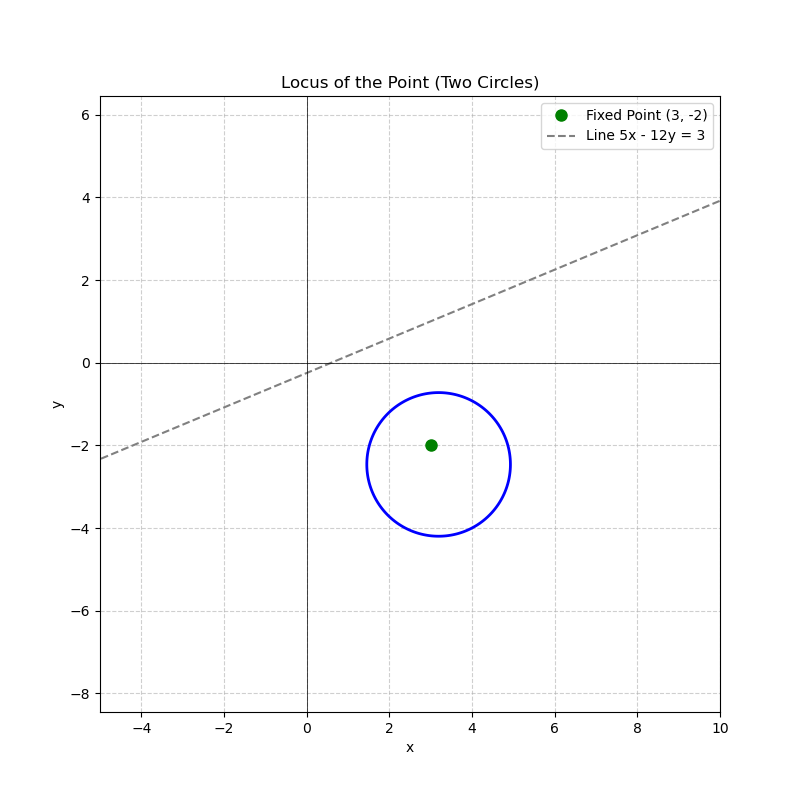
\includegraphics[width=0.6\linewidth]{Beamer/figs/circle.png}
    \caption{}
    \label{fig:placeholder}
\end{figure}

\end{frame}
\end{document}





